\documentclass[12pt,aspectratio=169]{beamer}
\usepackage{amsmath, amssymb}
\usepackage{booktabs}
\usepackage{tikz}
\usetikzlibrary{arrows.meta,decorations.pathmorphing,patterns}
\usepackage{pgfplots}
\pgfplotsset{compat=1.18}
\usepackage{xcolor}
\usepackage{array}

% ── Theme ──────────────────────────────────────────────────────────────
\usetheme{Madrid}
\definecolor{firered}{RGB}{180,30,10}
\definecolor{ashgrey}{RGB}{50,55,65}
\definecolor{skyblue}{RGB}{30,100,180}
\definecolor{flameyellow}{RGB}{230,155,15}
\setbeamercolor{palette primary}{bg=ashgrey,fg=white}
\setbeamercolor{palette secondary}{bg=ashgrey!85,fg=white}
\setbeamercolor{palette tertiary}{bg=ashgrey!65,fg=white}
\setbeamercolor{palette quaternary}{bg=ashgrey,fg=white}
\setbeamercolor{structure}{fg=skyblue}
\setbeamercolor{alerted text}{fg=firered}
\setbeamercolor{block title}{bg=skyblue,fg=white}
\setbeamercolor{block body}{bg=skyblue!8}
\setbeamercolor{block title alerted}{bg=firered,fg=white}
\setbeamercolor{block body alerted}{bg=firered!10}
\setbeamercolor{block title example}{bg=ashgrey,fg=white}
\setbeamercolor{block body example}{bg=ashgrey!10}
\setbeamerfont{title}{size=\Large,series=\bfseries}
\setbeamertemplate{navigation symbols}{}

% ── Macros ──────────────────────────────────────────────────────────────
\newcommand{\taures}{\tau}
\newcommand{\tchem}{t_{\text{chem}}}
\newcommand{\Da}{\mathrm{Da}}
\newcommand{\ddt}[1]{\frac{d#1}{dt}}
\newcommand{\Vr}{V}
\newcommand{\Tad}{T_{\text{ad}}}
\newcommand{\Tin}{T_{\text{in}}}
\newcommand{\Tout}{T_{\text{out}}}
\newcommand{\mdot}{\dot{m}}
\newcommand{\pd}[2]{\frac{\partial #1}{\partial #2}}
\newcommand{\Tt}{T_t}   % total temperature
\newcommand{\pt}{p_t}   % total pressure

% ════════════════════════════════════════════════════════════════════════
\title{The Well-Stirred Reactor}
\subtitle{Zero-Dimensional Combustion Theory for Aerospace Propulsion}
\author{Prof. Dr. Onur Tuncer}
\institute{UCK 427E Combustion }
\date{\today}

\begin{document}

\begin{frame}
  \titlepage
\end{frame}

\begin{frame}{Lecture Outline}
  \tableofcontents
\end{frame}

% ════════════════════════════════════════════════════════════════════════
\section{Motivation: Combustion in Aero-Engines}
% ════════════════════════════════════════════════════════════════════════

\begin{frame}{Where Does Combustion Live in an Aero-Engine?}
  \begin{center}
  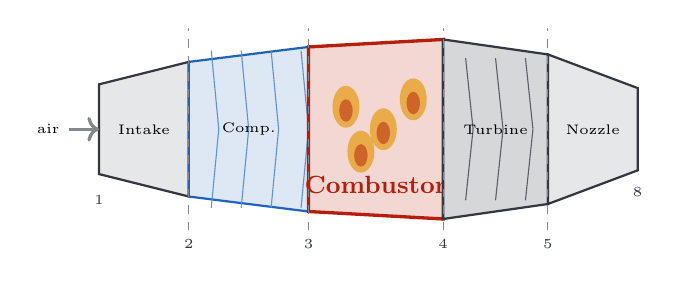
\begin{tikzpicture}[font=\small, scale=0.95]
    % Engine outline — simplified turbojet cross-section
    % Intake
    \draw[thick,ashgrey,fill=ashgrey!12]
      (0,0.6) -- (1.2,0.9) -- (1.2,-0.9) -- (0,-0.6) -- cycle;
    \node at (0.6,0) {\tiny Intake};

    % Compressor
    \draw[thick,skyblue,fill=skyblue!15]
      (1.2,0.9) -- (2.8,1.1) -- (2.8,-1.1) -- (1.2,-0.9) -- cycle;
    \foreach \x in {1.5,1.9,2.3,2.7}{
      \draw[skyblue!70,thin] (\x,1.05) -- (\x+0.1,0) -- (\x,-1.05);
    }
    \node at (2.0,0) {\tiny Comp.};

    % Combustor — highlighted
    \draw[very thick,firered,fill=firered!18]
      (2.8,1.1) -- (4.6,1.2) -- (4.6,-1.2) -- (2.8,-1.1) -- cycle;
    % flame symbols
    \foreach \cx/\cy in {3.3/0.3, 3.8/0.0, 4.2/0.4, 3.5/-0.3}{
      \fill[flameyellow,opacity=0.7] (\cx,\cy) ellipse (0.18 and 0.28);
      \fill[firered,opacity=0.5] (\cx,\cy-0.05) ellipse (0.09 and 0.15);
    }
    \node[firered,font=\small\bfseries] at (3.7,-0.75) {Combustor};

    % Turbine
    \draw[thick,ashgrey,fill=ashgrey!20]
      (4.6,1.2) -- (6.0,1.0) -- (6.0,-1.0) -- (4.6,-1.2) -- cycle;
    \foreach \x in {4.9,5.3,5.7}{
      \draw[ashgrey!80,thin] (\x,0.95) -- (\x+0.1,0) -- (\x,-0.95);
    }
    \node at (5.3,0) {\tiny Turbine};

    % Nozzle
    \draw[thick,ashgrey,fill=ashgrey!12]
      (6.0,1.0) -- (7.2,0.55) -- (7.2,-0.55) -- (6.0,-1.0) -- cycle;
    \node at (6.6,0) {\tiny Nozzle};

    % Station labels
    \foreach \x/\lab in {1.2/2, 2.8/3, 4.6/4, 6.0/5}{
      \draw[dashed,ashgrey!60] (\x,-1.35) -- (\x,1.35);
      \node[below,font=\tiny,ashgrey] at (\x,-1.35) {\lab};
    }
    \node[below,font=\tiny,ashgrey] at (0,-0.75) {1};
    \node[below,font=\tiny,ashgrey] at (7.2,-0.65) {8};

    % Flow arrow
    \draw[->,very thick,ashgrey!60] (-0.4,0) -- (0,0);
    \node[left,font=\tiny] at (-0.4,0) {air};
  \end{tikzpicture}
  \end{center}

  \medskip
  \begin{columns}
    \begin{column}{0.48\textwidth}
      \textbf{Main combustor} (stations 3$\to$4):
      compressed air + Jet-A, $p\sim15$--$40$ bar, $T_3\sim700$--$900$ K,
      $\taures \sim 3$--$8$ ms.
    \end{column}
    \begin{column}{0.48\textwidth}
      \textbf{Afterburner / reheat} (stations 5$\to$8):
      turbine exit gas + extra fuel, $p\sim2$--$5$ bar, very short
      $\taures \sim 1$--$3$ ms --- extreme blowout risk.
    \end{column}
  \end{columns}
\end{frame}

\begin{frame}{Why a Simple Model? The Modelling Hierarchy}

  \begin{center}
  \renewcommand{\arraystretch}{1.35}
  \begin{tabular}{>{\bfseries}p{3.5cm} p{4.0cm} p{4.0cm}}
    \toprule
    Model & Cost & Use in propulsion \\
    \midrule
    \alert{0-D WSR} & $< 1$ s & Stability limits, fuel screening,
                                  mechanism validation \\
    1-D network     & seconds  & Multi-zone combustor sizing \\
    RANS CFD        & hours    & Flow fields, cooling design \\
    LES / DNS       & days--weeks & Instability, NOx, soot \\
    \bottomrule
  \end{tabular}
  \end{center}

  \medskip
  \begin{block}{The role of the WSR}
    Sits at the \textbf{base} of the hierarchy.
    Captures the essential competition between \emph{residence time} and
    \emph{chemical time} at negligible cost.
    Every preliminary combustor design starts here.
  \end{block}
\end{frame}

% ════════════════════════════════════════════════════════════════════════
\section{The Zero-Dimensional Idealisation}
% ════════════════════════════════════════════════════════════════════════

\begin{frame}{Zero-Dimensional: Collapsing Space to a Point}

  \begin{columns}
    \begin{column}{0.56\textwidth}
      A \textbf{zero-dimensional (0-D)} model replaces all spatial variation
      with a \emph{single uniform state}:

      \medskip
      \begin{block}{Mathematical statement}
        For \emph{any} scalar field $\phi(\mathbf{x},t)$ inside $\Vr$:
        \[
          \phi(\mathbf{x},t) \equiv \phi(t) \qquad \forall\,\mathbf{x} \in \Vr
        \]
        \textbf{All spatial gradients are identically zero.}
        No convection, no diffusion, no spatial operators.
      \end{block}

      \medskip
      PDEs $\longrightarrow$ \textbf{coupled ODEs} in time.
      At steady state $\longrightarrow$ \textbf{algebraic equations}.
    \end{column}
    \begin{column}{0.41\textwidth}
      \centering
      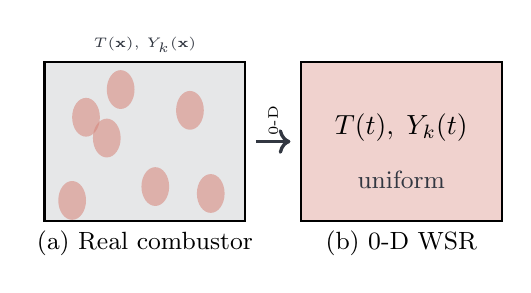
\begin{tikzpicture}[scale=0.88, font=\small]
        % Real combustor
        \draw[thick,fill=ashgrey!12] (0,0) rectangle (2.9,2.3);
        \foreach \x/\y in {0.4/0.3, 0.9/1.2, 1.6/0.5, 2.1/1.6,
                            1.1/1.9, 2.4/0.4, 0.6/1.5}{
          \fill[firered!55,opacity=0.55] (\x,\y) ellipse (0.2 and 0.28);
        }
        \node at (1.45,-0.32) {\small (a) Real combustor};
        \node[font=\tiny,ashgrey] at (1.45,2.55) {$T(\mathbf{x}),\,Y_k(\mathbf{x})$};

        % Arrow
        \draw[->,very thick,ashgrey] (3.05,1.15) -- (3.55,1.15);
        \node[font=\tiny,rotate=90] at (3.3,1.45) {0-D};

        % 0-D box
        \draw[thick,fill=firered!20] (3.7,0) rectangle (6.6,2.3);
        \node[font=\normalsize] at (5.15,1.35) {$T(t),\;Y_k(t)$};
        \node[font=\small,ashgrey] at (5.15,0.6) {uniform};
        \node at (5.15,-0.32) {\small (b) 0-D WSR};
      \end{tikzpicture}
    \end{column}
  \end{columns}
\end{frame}

\begin{frame}{Physical Realisation: The Well-Stirred Reactor}

  The 0-D idealisation is physically realised as the
  \alert{Well-Stirred Reactor (WSR)} --- also called a
  \textit{Perfectly Stirred Reactor} (PSR) or
  \textit{Longwell Reactor} in the combustion literature.

  \medskip
  \textbf{Validity conditions:}
  \begin{enumerate}
    \item $t_{\text{mix}} \ll \tchem$ \quad
          (mixing faster than reaction --- no flame sheets inside)
    \item $t_{\text{mix}} \ll \taures$ \quad
          (mixing faster than throughflow)
    \item No temperature or composition gradients inside $\Vr$
  \end{enumerate}

  \medskip
  \begin{alertblock}{Critical consequence}
    Reaction rates are evaluated at the \textbf{hot, burned} exit state ---
    not at the cold inlet.
    This is why the WSR sustains combustion at conditions where a cold-flow
    reactor would extinguish.
  \end{alertblock}

  \begin{exampleblock}{In practice}
    Gas turbine primary zones achieve WSR-like behaviour via strong swirl
    and recirculation ($t_{\text{mix}} \sim 0.1$--$0.5$ ms).
  \end{exampleblock}
\end{frame}

\begin{frame}{What the 0-D Assumption Eliminates}

  \begin{columns}[t]
    \begin{column}{0.49\textwidth}
      \textbf{Full reactive Navier--Stokes (3-D)}
      \begin{align*}
        \pd{\rho}{t} &+ \nabla\cdot(\rho\mathbf{u}) = 0\\[2pt]
        \pd{(\rho Y_k)}{t} &+ \nabla\cdot(\rho\mathbf{u}Y_k)
          = \nabla\cdot(\rho D_k \nabla Y_k) + \dot{\omega}_k W_k\\[2pt]
        \rho c_p\pd{T}{t} &+ \rho c_p\mathbf{u}\cdot\nabla T
          = \nabla\cdot(\lambda\nabla T) - \textstyle\sum_k h_k \dot{\omega}_k W_k
      \end{align*}
      \vspace{0.5em}
      \small Millions of DOF in a real combustor CFD.
    \end{column}
    \begin{column}{0.49\textwidth}
      \textbf{0-D WSR \quad($\nabla \equiv \mathbf{0}$)}
      \begin{align*}
        \Vr\ddt{(\rho Y_k)}
          &= \mdot_{\text{in}}(Y_{k,\text{in}}-Y_k)
            + \dot{\omega}_k W_k \Vr \\[8pt]
        \Vr \rho c_p \ddt{T}
          &= \mdot_{\text{in}} c_p(\Tin-T)\\
          &\quad - \textstyle\sum_k h_k \dot{\omega}_k W_k \Vr
      \end{align*}
      \vspace{0.5em}
      \small \textbf{One point.} Seconds to solve.
    \end{column}
  \end{columns}

  \medskip
  \begin{block}{The payoff}
    All spatial operators vanish.  A combustor modelled with $10^6$ CFD cells
    collapses to \textbf{a single algebraic system}.
    Ideal for: preliminary design, stability maps, fuel/altitude sweeps,
    kinetic mechanism validation.
  \end{block}
\end{frame}

% ════════════════════════════════════════════════════════════════════════
\section{Ideal Gas in an Aero-Engine Combustor}
% ════════════════════════════════════════════════════════════════════════

\begin{frame}{Ideal Gas Law in a Combustor}

  All combustion products (N$_2$, O$_2$, CO$_2$, H$_2$O, \ldots) obey:
  \[
    p = \rho R_u T \sum_k \frac{Y_k}{W_k} \equiv \rho \bar{R} T
    \qquad \Rightarrow \qquad
    \rho = \frac{p\bar{W}}{R_u T}
  \]

  \begin{columns}[t]
    \begin{column}{0.50\textwidth}
      \textbf{Isobaric combustor (main burner)}\\[4pt]
      Neglect $\Delta p$ across the flame ($\Delta p/p \sim 3$--$5\%$):
      \[
        p \approx p_3 = \text{const}
        \quad\Rightarrow\quad
        \frac{\rho_3}{\rho_4} = \frac{T_4}{T_3} \approx 2\text{--}3
      \]
      Hot gas expands by a factor $\sim T_4/T_3$ ---
      exit velocity is $\sim 2$--$3\times$ inlet velocity.
    \end{column}
    \begin{column}{0.46\textwidth}
      \textbf{Jet-A global reaction}\\[4pt]
      Approximate stoichiometry:
      \[
        \text{C}_{12}\text{H}_{23} + 17.75\,\text{O}_2
        \to 12\,\text{CO}_2 + 11.5\,\text{H}_2\text{O}
      \]
      Global rate (Westbrook \& Dryer):
      \[
        \dot{\omega}_F \!=\! A\,e^{-E_a/R_u T}
        [\text{C}_{12}\text{H}_{23}]^{0.25}[\text{O}_2]^{1.5}
      \]
      $E_a/R_u \approx 15{,}000$ K for Jet-A.
    \end{column}
  \end{columns}
\end{frame}

\begin{frame}{Inlet Conditions Across the Flight Envelope}

  Station 3 (combustor inlet) conditions depend on flight Mach number $M$
  and altitude $H$.  From isentropic relations:
  \[
    T_3 = T_0\left(1 + \frac{\gamma-1}{2}M^2\right)\!\eta_c^{-1}\,\pi_c^{(\gamma-1)/\gamma},
    \qquad
    p_3 = p_0\left(\frac{T_3}{T_0}\right)^{\gamma/(\gamma-1)}
  \]

  \medskip
  \renewcommand{\arraystretch}{1.3}
  \begin{tabular}{lcccccc}
    \toprule
    Condition & $H$ (km) & $M$ & $T_0$ (K) & $p_0$ (kPa) & $T_3$ (K) & $p_3$ (bar) \\
    \midrule
    Sea-level static & 0   & 0   & 288 & 101 & 780 & 38 \\
    Cruise (civil)   & 11  & 0.85& 217 & 23  & 700 & 17 \\
    Cruise (combat)  & 11  & 0.9 & 217 & 23  & 710 & 20 \\
    Low-level fast   & 0   & 0.9 & 288 & 101 & 840 & 55 \\
    High alt.\ dash  & 18  & 1.5 & 217 & 7   & 630 & 8  \\
    \bottomrule
  \end{tabular}

  \medskip
  \small ($\pi_c \approx 15$ for civil; $\approx 25$ for combat.
  Conditions strongly affect $\taures$ and blowout margin.)
\end{frame}

% ════════════════════════════════════════════════════════════════════════
\section{Residence Time}
% ════════════════════════════════════════════════════════════════════════

\begin{frame}{Residence Time: Definition \& Ideal-Gas Form}

  \begin{block}{Definition (mass-based)}
    \[
      \taures = \frac{m_{\text{gas in combustor}}}{\mdot_{\text{air}}}
      = \frac{\rho(\Tout,\,p)\,\Vr}{\mdot_{\text{air}}}
    \]
  \end{block}

  Substituting ideal gas $\rho = p\bar{W}/(R_u \Tout)$:
  \[
    \boxed{
      \taures = \frac{p\,\bar{W}\,\Vr}{R_u\,\Tout\,\mdot_{\text{air}}}
    }
  \]

  \begin{columns}[t]
    \begin{column}{0.50\textwidth}
      \textbf{Key coupling}\\[4pt]
      $\taures$ depends on \alert{reactor temperature $\Tout$}.
      Hotter combustion $\Rightarrow$ lower $\rho$ $\Rightarrow$
      shorter $\taures$ for the same $\mdot$.
    \end{column}
    \begin{column}{0.46\textwidth}
      \textbf{Altitude effect (fixed $\Vr$, fixed $\mdot$)}\\[4pt]
      \[
        \taures \propto \frac{p}{\Tout}
      \]
      At cruise altitude $p$ drops $\sim 4\times$
      $\Rightarrow$ $\taures$ shrinks $\sim 4\times$
      $\Rightarrow$ blowout risk $\uparrow$
    \end{column}
  \end{columns}
\end{frame}

\begin{frame}{Combustor Loading Parameter}

  In gas turbine practice, $\taures$ is captured by the
  \alert{combustor loading parameter} $\mathcal{L}$
  (Lefebvre notation):
  \[
    \mathcal{L} = \frac{\mdot_{\text{air}}}{p^n\,\Vr}
    \qquad n \approx 1.8 \text{ (empirical)}
  \]

  \begin{itemize}
    \item High $\mathcal{L}$: high flow per unit volume $\to$ short $\taures$
          $\to$ blowout risk.
    \item Low $\mathcal{L}$: long $\taures$, high efficiency, risk of hot spots
          and soot.
    \item Design constraint: $\mathcal{L}_{\text{idle}} \leq \mathcal{L}
          \leq \mathcal{L}_{\text{max}}$ over the entire flight envelope.
  \end{itemize}

  \begin{exampleblock}{Typical values (annular combustors)}
    \begin{tabular}{lc}
      Civil turbofan (cruise) & $\mathcal{L} \approx 20$--$50$ kg/(s$\cdot$atm$^{1.8}$m$^3$)\\
      Military afterburner    & $\mathcal{L} \approx 500$--$2000$ \\
    \end{tabular}
  \end{exampleblock}
\end{frame}

\begin{frame}{Chemical Time Scale \& the Damk\"{o}hler Number}

  \textbf{Chemical time} for fuel consumption:
  \[
    \tchem = \frac{\rho Y_{F,\text{in}}}{|\dot{\omega}_F| W_F}
    \sim \frac{1}{A\,e^{-E_a/R_u T}\,[\text{O}_2]^n}
  \]
  Strongly temperature-dependent via the Arrhenius exponential.

  \medskip
  \begin{block}{Damk\"{o}hler Number}
    \[
      \Da = \frac{\taures}{\tchem}
      = \frac{\text{time available for reaction}}{\text{time chemistry needs}}
    \]
  \end{block}

  \begin{center}
  \renewcommand{\arraystretch}{1.3}
  \begin{tabular}{cll}
    \toprule
    $\Da$ & Chemistry regime & Combustor behaviour \\
    \midrule
    $\gg 1$ & Fast chemistry & Full burning, $\eta_c \to 1$, $T \to \Tad$ \\
    $\sim 1$ & Finite-rate effects & Partial burn, CO/UHC emissions \\
    $\ll 1$ & Slow chemistry & \alert{Blowout / flame extinction} \\
    \bottomrule
  \end{tabular}
  \end{center}
\end{frame}

% ════════════════════════════════════════════════════════════════════════
\section{Steady-State Analysis \& the S-Curve}
% ════════════════════════════════════════════════════════════════════════

\begin{frame}{Steady-State Balances}

  At steady state, the 0-D equations become algebraic.

  \textbf{Species (fuel):}
  \[
    \frac{Y_{F,\text{in}} - Y_F}{\taures} = \frac{|\dot{\omega}_F| W_F}{\rho}
  \]

  \textbf{Energy (adiabatic):}
  \[
    \Tout = \Tin + \frac{Q_{\text{HV}}(Y_{F,\text{in}}-Y_F)}{c_p}
          = \Tin + \eta_c\,\Delta T_{\text{ad}}
  \]

  where $\eta_c = (Y_{F,\text{in}}-Y_F)/Y_{F,\text{in}}$ is the
  \textbf{combustion efficiency} and
  $\Delta T_{\text{ad}} = Q_{\text{HV}}\,Y_{F,\text{in}}/c_p$.

  \begin{alertblock}{Non-linearity}
    $\taures$ depends on $\Tout$ (ideal gas), and $\dot{\omega}_F$ depends
    exponentially on $\Tout$.  The system is \textbf{highly non-linear}
    $\to$ multiple solutions possible.
  \end{alertblock}
\end{frame}

\begin{frame}{The S-Curve: Heart of Combustor Stability Theory}

  \begin{columns}
    \begin{column}{0.50\textwidth}
      Parametric solution traces an \alert{S-shaped curve}
      in the $(\taures,\,T)$ or $(\taures,\,\eta_c)$ plane.

      \medskip
      \begin{itemize}
        \item \textbf{\textcolor{firered}{Upper branch}}:
              fully burning; $T \approx \Tad$, $\eta_c \approx 1$
        \item \textbf{Lower branch} (grey):
              essentially unburned; $T \approx \Tin$
        \item \textbf{Middle branch} (dashed):
              mathematically unstable --- never observed
        \item \textbf{Lower turning point}: \alert{Blowout limit}
              $\taures_{\text{bo}}$
        \item \textbf{Upper turning point}: Ignition limit
              $\taures_{\text{ign}}$
      \end{itemize}
    \end{column}
    \begin{column}{0.47\textwidth}
      \centering
      
\begin{tikzpicture}
        \begin{axis}[
            width=\textwidth, height=0.64\textheight,
            xlabel={Residence time $\taures$},
            ylabel={Reactor temperature $T$},
            xtick={1.05,2.55},
            xticklabels={$\taures_{\text{bo}}$, $\taures_{\text{ign}}$},
            ytick={0.12,0.88},
            yticklabels={$T_{\text{in}}$, $T_{\text{ad}}$},
            xmin=0.2, xmax=5.5, ymin=0, ymax=1.05,
            samples=400, thick, clip=false,
        ]
          % Upper branch (burning)
          \addplot[firered,very thick,domain=1.05:5.3]
            ({x},{0.87 - 0.05*(x-2.8)^2/(1+(x-2.8)^2)
                      + 0.03*exp(-6*(x-1.3)^2)});
          % Lower branch (unburned)
          \addplot[ashgrey,thick,domain=0.3:5.3]
            ({x},{0.11 + 0.025/x});
          % Unstable middle branch
          \addplot[ashgrey!50,dashed,very thick,domain=1.05:2.55]
            ({x},{0.13 + 0.36*(x-1.05)/(2.55-1.05)});

          % Blowout marker
          \node[circle,fill=firered,inner sep=3.2pt] at (axis cs:1.05,0.88){};
          \draw[->,thick,firered] (axis cs:1.05,0.88)
            -- (axis cs:1.05,0.13) node[below,firered,font=\small]{\textbf{Blowout}};

          % Ignition marker
          \node[circle,fill=flameyellow!90!black,inner sep=3.2pt]
            at (axis cs:2.55,0.49){};
          \draw[<-,thick,flameyellow!80!black]
            (axis cs:2.55,0.49) -- (axis cs:3.8,0.35)
            node[right,font=\small]{Ignition};

          % Arrow showing direction of decreasing tau
          \draw[->,thick,firered!60]
            (axis cs:4.6,0.95) -- (axis cs:1.8,0.95)
            node[midway,above,font=\tiny]{decrease $\taures$
                                          (increase $\mdot$ or reduce $p$)};
        \end{axis}
      \end{tikzpicture}
    \end{column}
  \end{columns}
\end{frame}

% ════════════════════════════════════════════════════════════════════════
\section{Blowout}
% ════════════════════════════════════════════════════════════════════════

\begin{frame}{Blowout: Physical Mechanism}

  \begin{columns}
    \begin{column}{0.58\textwidth}
      \textbf{Blowout} (or \textit{blowoff}) is the abrupt extinction of the
      flame when residence time falls below the critical value
      $\taures_{\text{bo}}$:
      \[
        \taures < \taures_{\text{bo}}
        \quad\Leftrightarrow\quad
        \Da < \Da_{\text{crit}} \approx 1
      \]

      \medskip
      \textbf{Positive-feedback extinction cascade:}
      \begin{enumerate}
        \item $\mdot \uparrow$ or $p \downarrow$
              $\;\Rightarrow\;$ $\taures \downarrow$
        \item Incomplete combustion: $T\downarrow$, $\eta_c \downarrow$
        \item Arrhenius: $\dot{\omega}_F \propto e^{-E_a/R_u T}$
              drops \emph{exponentially}
        \item Less heat $\Rightarrow$ further $T\downarrow$
        \item \alert{Flame extinguishes abruptly} (fold bifurcation)
      \end{enumerate}

      \medskip
      In an aero-engine: sudden loss of thrust, potential surge,
      unburned fuel in hot section --- \textbf{critical safety event.}
    \end{column}
    \begin{column}{0.38\textwidth}
      \centering
      
\begin{tikzpicture}
        \begin{axis}[
            width=\textwidth, height=0.65\textheight,
            xlabel={$\taures$},
            ylabel={$T_{\text{reactor}}$},
            xtick={1.0}, xticklabels={$\taures_{\text{bo}}$},
            ytick=\empty,
            xmin=0.2, xmax=4.5, ymin=0, ymax=1.05,
            samples=300, thick,
        ]
          \addplot[firered,very thick,domain=1.0:4.4]
            ({x},{0.86+0.03*exp(-5*(x-1.0)^2)});
          \addplot[ashgrey,thick,domain=0.2:4.4]
            ({x},{0.10+0.02/x});
          \addplot[ashgrey!50,dashed,domain=1.0:2.3]
            ({x},{0.12+0.38*(x-1.0)});
          \node[circle,fill=firered,inner sep=3.5pt]
            at (axis cs:1.0,0.86){};
          \draw[->,ultra thick,firered!80]
            (axis cs:1.0,0.86) -- (axis cs:1.0,0.11);
          \node[right,font=\tiny,firered] at (axis cs:1.02,0.50)
            {\textbf{blowout} drop};
          \draw[->,thick,ashgrey!50]
            (axis cs:3.8,0.93)--(axis cs:1.5,0.93)
            node[midway,above,font=\tiny]{$\taures\downarrow$};
        \end{axis}
      \end{tikzpicture}
    \end{column}
  \end{columns}
\end{frame}

\begin{frame}{Blowout Criterion: Longwell--Weiss Analysis}

  Balance heat release against enthalpy carried out of the reactor.

  \medskip
  \textbf{Volumetric heat release rate:}
  \[
    \dot{q}''' = Q_{\text{HV}}\,|\dot{\omega}_F|\,W_F
    = Q_{\text{HV}}\,A\,e^{-E_a/R_u T}\,
      \left(\frac{p\bar{W}}{R_u T}\right)^{m+n}
      Y_F^m Y_{\text{ox}}^n
  \]

  \textbf{Enthalpy removal rate (per unit volume):}
  \[
    \dot{q}_{\text{rem}}''' = \frac{\rho c_p (T-\Tin)}{\taures}
  \]

  \begin{alertblock}{Blowout: tangency condition}
    \[
      \dot{q}''' = \dot{q}_{\text{rem}}'''
      \quad \text{and} \quad
      \frac{d\dot{q}'''}{dT} = \frac{d\dot{q}_{\text{rem}}'''}{dT}
    \]
    The S-curve folds back --- two solutions merge and disappear.
  \end{alertblock}
\end{frame}

\begin{frame}{Critical Residence Time \& Pressure Scaling}

  For a one-step global reaction at blowout temperature
  $T_{\text{bo}} \approx 0.75$--$0.85\,\Tad$:

  \[
    \taures_{\text{bo}}
    \approx \frac{\rho_{\text{bo}}\,c_p\,(T_{\text{bo}}-\Tin)}
    {Q_{\text{HV}}\,A\,e^{-E_a/R_u T_{\text{bo}}}
     \,[\text{Fuel}]^m[\text{O}_2]^n}
  \]

  With ideal gas $\rho \propto p/T$, for $m+n \approx 1.75$ (Jet-A):
  \[
    \boxed{
      \taures_{\text{bo}} \propto \frac{T_{\text{bo}}}{p^{0.75}}\,
      e^{+E_a/R_u T_{\text{bo}}}
    }
  \]

  \begin{columns}[t]
    \begin{column}{0.50\textwidth}
      \textbf{Design implications}
      \begin{itemize}
        \item $p \downarrow$ (altitude): $\taures_{\text{bo}} \uparrow$
              --- need larger $\Vr$ or lower $\mdot$
        \item Lean ($\phi \downarrow$): $T_{\text{bo}} \downarrow$,
              exponentially longer $\taures_{\text{bo}}$
        \item High $E_a$ fuels: stronger altitude sensitivity
      \end{itemize}
    \end{column}
    \begin{column}{0.46\textwidth}
      \begin{exampleblock}{Order of magnitude (Jet-A)}
        \begin{tabular}{lc}
          \small Condition & $\taures_{\text{bo}}$ \\
          \midrule
          S/L, $\phi=0.8$, $T_3=700$K & $\sim 1$--$2$ ms \\
          $H=11$km, $\phi=0.5$ & $\sim 5$--$15$ ms \\
          Afterburner ($T_5\sim900$K) & $\sim 0.5$--$1$ ms \\
        \end{tabular}
      \end{exampleblock}
    \end{column}
  \end{columns}
\end{frame}

\begin{frame}{Blowout Across the Flight Envelope}

  \begin{columns}
    \begin{column}{0.52\textwidth}
      \centering
      \begin{tikzpicture}
        \begin{axis}[
            width=\textwidth, height=0.70\textheight,
            xlabel={Mach number $M$},
            ylabel={Altitude $H$ (km)},
            xmin=0, xmax=2.5, ymin=0, ymax=20,
            xtick={0,0.5,1.0,1.5,2.0,2.5},
            ytick={0,5,10,15,20},
            grid=major,
            thick,
        ]
          % Safe operating region (shaded)
          \addplot[skyblue!30,fill=skyblue!20,fill opacity=0.7]
            coordinates{(0,0)(2.5,0)(2.5,10)(2.0,14)(1.5,17)(0.5,18)(0,18)(0,0)};
          \addlegendentry{Stable combustion}

          % Blowout boundary
          \addplot[firered,very thick,domain=0:2.5]
            ({x},{17.5 - 3.5*x - 1.5*x^2 + 0.5*x^3});
          \addlegendentry{Blowout boundary}

          % Rich blowout (low alt, high speed -- less relevant, show as dashed)
          \addplot[flameyellow!80!black,dashed,thick]
            coordinates{(1.8,0)(2.5,6)};
          \addlegendentry{Rich blowout (A/B)}

          % Labels
          \node[font=\small,skyblue!60!black] at (axis cs:1.0,7)
            {Operating envelope};
          \node[font=\small,firered] at (axis cs:0.5,19.2)
            {Lean blowout};
        \end{axis}
      \end{tikzpicture}
    \end{column}
    \begin{column}{0.44\textwidth}
      \textbf{Why the boundary exists}
      \begin{itemize}
        \item At high altitude: $p \downarrow$ $\Rightarrow$
              $\tchem \uparrow$, $\taures \downarrow$,
              $\Da \downarrow \to \Da_{\text{crit}}$
        \item At low-level / high speed: $\mdot \uparrow$
              $\Rightarrow$ $\taures \downarrow$
        \item Afterburner: low $p_5$, short combustor ---
              blowout boundary very restrictive
      \end{itemize}

      \medskip
      \textbf{Mitigation strategies}
      \begin{itemize}
        \item Pilot / torch igniters for relight
        \item Variable-geometry combustor dilution holes
        \item Swirl-stabilised recirculation zone
              (increases effective $\taures$)
        \item Staged combustion (RQL)
      \end{itemize}
    \end{column}
  \end{columns}
\end{frame}

\begin{frame}{Afterburner Blowout: A Special Challenge}

  \begin{columns}[t]
    \begin{column}{0.54\textwidth}
      The afterburner (reheat) system operates under the most demanding
      conditions in the propulsion system:

      \medskip
      \begin{tabular}{lcc}
        \toprule
        Parameter & Main burner & Afterburner \\
        \midrule
        $p$ (bar) & 15--40 & 2--5 \\
        $T_{\text{in}}$ (K) & 700--900 & 800--1000 \\
        $\taures$ (ms) & 3--8 & 0.5--2 \\
        $\phi$ & 0.3--0.6 & 0.4--1.2 \\
        \bottomrule
      \end{tabular}

      \medskip
      Low $p$ + short $\taures$ + cold gas dilution makes lean blowout
      the dominant failure mode.
    \end{column}
    \begin{column}{0.42\textwidth}
      \textbf{Gutter flameholder WSR model}\\[6pt]
      The recirculation zone behind a V-gutter is modelled as a WSR:
      \[
        \Vr_{\text{rec}} \approx 0.38\,w\,h\,L_g
      \]
      where $w$, $h$ are gutter dimensions.

      \medskip
      Blowout occurs when:
      \[
        \frac{\mdot_{\text{air,rec}}}
             {\Vr_{\text{rec}}\,p^{1.8}}
        > \mathcal{L}_{\text{bo}}(\phi,\,T_{\text{in}})
      \]

      Increasing $L_g$ (longer gutter) increases $\Vr_{\text{rec}}$
      and delays blowout.
    \end{column}
  \end{columns}
\end{frame}

\begin{frame}{Equivalence Ratio \& Blowout Stability Loop}

  \centering
  \begin{tikzpicture}
    \begin{axis}[
        width=0.72\textwidth, height=0.60\textheight,
        xlabel={Equivalence ratio $\phi$},
        ylabel={$\mdot_{\text{bo}}\,/\,(p^{1.8}\Vr)$ \quad [stability margin]},
        xmin=0.3, xmax=1.6,
        ymin=0, ymax=1.25,
        samples=200, domain=0.35:1.55,
        xtick={0.5,1.0,1.4},
        xticklabels={lean limit, stoich, rich limit},
        ytick=\empty,
        grid=major, thick,
    ]
      \addplot[firered,very thick]{1.1*exp(-3.5*(x-1.0)^2)};
      \addplot[ashgrey,dashed,thick] coordinates{(1.0,0)(1.0,1.1)};
      \node[above,font=\small] at (axis cs:1.0,1.1){peak stability};

      % Lean blowout zone
      \addplot[firered!15,fill=firered!15,fill opacity=0.7,domain=0.35:0.55]
        {1.1*exp(-3.5*(x-1.0)^2)} \closedcycle;
      \node[firered,font=\small] at (axis cs:0.44,0.45){lean blowout};

      % Rich blowout zone
      \addplot[firered!15,fill=firered!15,fill opacity=0.7,domain=1.35:1.55]
        {1.1*exp(-3.5*(x-1.0)^2)} \closedcycle;
      \node[firered,font=\small] at (axis cs:1.46,0.45){rich blowout};

      % Operating point markers
      \node[circle,fill=skyblue,inner sep=3pt] at (axis cs:0.6,0.75){};
      \node[right,font=\tiny,skyblue] at (axis cs:0.62,0.75){LPP cruise};
      \node[circle,fill=skyblue,inner sep=3pt] at (axis cs:0.8,1.0){};
      \node[right,font=\tiny,skyblue] at (axis cs:0.82,1.0){RQL primary};
    \end{axis}
  \end{tikzpicture}

  \small Blowout mass flow rate peaks near stoichiometric (most stable).
  Modern low-NO$_x$ LPP designs operate near the lean limit ---
  small margin to blowout.
\end{frame}

\begin{frame}{Combustor Design Strategies vs.\ Blowout}

  \begin{columns}[t]
    \begin{column}{0.49\textwidth}
      \textbf{Rich--Quench--Lean (RQL)}
      \begin{itemize}
        \item Primary zone: $\phi \sim 1.5$--$1.8$, rich and well away from lean blowout
        \item Quick-quench jets $\to$ lean $\phi < 0.5$
        \item \textit{Pro}: robust against blowout
        \item \textit{Con}: NO$_x$ spike in quench zone
      \end{itemize}
    \end{column}
    \begin{column}{0.49\textwidth}
      \textbf{Lean Premixed Prevaporised (LPP)}
      \begin{itemize}
        \item Entire primary zone at $\phi \approx 0.5$--$0.65$
        \item Very low NO$_x$ ($<10$ EI)
        \item \textit{Pro}: low emissions
        \item \textit{Con}: very close to lean blowout; needs pilot flame at throttle-back
      \end{itemize}
    \end{column}
  \end{columns}

  \medskip
  \begin{block}{WSR as a design tool}
    Given target $\phi$, $\Tin$, and $p$ range, use the WSR blowout
    correlation to size $\Vr_c$ such that:
    \[
      \taures_{\text{design}} \geq k_{\text{safety}}\,\taures_{\text{bo}}
      \qquad k_{\text{safety}} \approx 2\text{--}4
    \]
    Typical preliminary design step before CFD.
  \end{block}
\end{frame}

% ════════════════════════════════════════════════════════════════════════
\section{Transient Response \& Relight}
% ════════════════════════════════════════════════════════════════════════

\begin{frame}{Transient 0-D Equations}

  Full unsteady WSR (constant $\Vr$, isobaric):
  \begin{align}
    \ddt{Y_k} &= \frac{Y_{k,\text{in}}-Y_k}{\taures}
                 + \frac{\dot{\omega}_k W_k}{\rho} \\[8pt]
    \ddt{T}   &= \frac{\Tin-T}{\taures}
                 - \frac{1}{\rho c_p}\sum_k h_k \dot{\omega}_k W_k
  \end{align}

  \begin{columns}[t]
    \begin{column}{0.50\textwidth}
      \textbf{Numerical aspects}
      \begin{itemize}
        \item Stiff system: $\taures \sim$ ms, elementary steps $\sim$ ns
        \item Implicit solvers: CVODE, \texttt{ode15s}, BDF
        \item Detailed mechanisms (GRI-Mech 3.0: 53 species, 325 reactions)
              are tractable at 0-D
      \end{itemize}
    \end{column}
    \begin{column}{0.46\textwidth}
      \textbf{Aero-engine transients}
      \begin{itemize}
        \item Throttle snap-back $\to$ lean transient
        \item Compressor surge $\to$ pressure drop, reduced $\taures$
        \item High-altitude relight: cold inlet, low $p$
        \item Windmill relight envelope bounded by 0-D blowout/ignition map
      \end{itemize}
    \end{column}
  \end{columns}
\end{frame}

\begin{frame}{Ignition \& Relight Hysteresis}

  For a combustor initially cold ($T \approx \Tin$),
  ignition requires $\taures > \taures_{\text{ign}}$.

  \[
    \taures_{\text{ign}} > \taures_{\text{bo}}
    \quad \Rightarrow \quad
    \text{\textbf{hysteresis window}}
  \]

  \begin{columns}
    \begin{column}{0.55\textwidth}
      \begin{itemize}
        \item Once burning at $\taures_{\text{bo}} < \taures < \taures_{\text{ign}}$:
              \emph{combustion is sustained}
        \item From cold: \emph{no ignition} at the same $\taures$
        \item Windmill relight must achieve $\taures > \taures_{\text{ign}}$
              (lower engine speed $\Rightarrow$ longer $\taures$)
        \item FADEC logic uses this hysteresis map to schedule relight
              attempts
      \end{itemize}
    \end{column}
    \begin{column}{0.41\textwidth}
      \begin{exampleblock}{Hysteresis on S-curve}
        \centering
        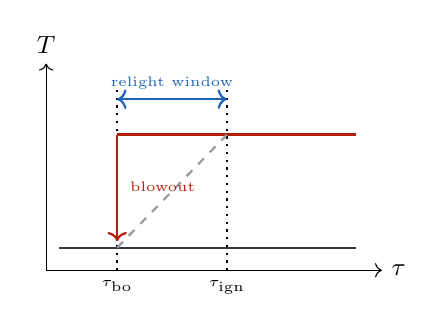
\begin{tikzpicture}[font=\small,scale=0.82]
          \draw[->] (0,0) -- (5.2,0) node[right]{$\taures$};
          \draw[->] (0,0) -- (0,3.2) node[above]{$T$};
          \draw[dotted,thick] (1.1,0)
            node[below,font=\tiny]{$\tau_{\text{bo}}$} -- (1.1,2.8);
          \draw[dotted,thick] (2.8,0)
            node[below,font=\tiny]{$\tau_{\text{ign}}$} -- (2.8,2.8);
          % burning branch
          \draw[firered,very thick] (1.1,2.1) -- (4.8,2.1);
          % unburned
          \draw[ashgrey,thick] (0.2,0.35) -- (4.8,0.35);
          % unstable
          \draw[dashed,ashgrey!50,thick] (1.1,0.35) -- (2.8,2.1);
          % hysteresis arrow
          \draw[<->,thick,skyblue] (1.1,2.65) -- (2.8,2.65)
            node[midway,above,font=\tiny]{relight window};
          % blowout arrow
          \draw[->,thick,firered] (1.1,2.1) -- (1.1,0.45);
          \node[right,font=\tiny,firered] at (1.15,1.3){blowout};
        \end{tikzpicture}
      \end{exampleblock}
    \end{column}
  \end{columns}
\end{frame}

% ════════════════════════════════════════════════════════════════════════
\section{Summary \& Design Implications}
% ════════════════════════════════════════════════════════════════════════

\begin{frame}{Key Equations at a Glance}
  \renewcommand{\arraystretch}{1.6}
  \begin{tabular}{>{\bfseries}p{4.2cm} p{7.5cm}}
    \toprule
    Concept & Expression \\
    \midrule
    0-D assumption & $\phi(\mathbf{x},t) = \phi(t)$; all $\nabla \equiv \mathbf{0}$ \\
    Residence time (ideal gas) &
      $\taures = p\bar{W}\Vr\,/\,(R_u\Tout\,\mdot_{\text{air}})$ \\
    Species balance (SS) &
      $(Y_{k,\text{in}}-Y_k)/\taures = |\dot{\omega}_k|W_k/\rho$ \\
    Energy balance (SS, adiab.) &
      $\Tout = \Tin + \eta_c\,Q_{\text{HV}}\,Y_{F,\text{in}}/c_p$ \\
    Damk\"{o}hler & $\Da = \taures/\tchem$; blowout at $\Da \sim 1$ \\
    Blowout scaling &
      $\taures_{\text{bo}} \propto (T_{\text{bo}}/p^{0.75})\,
        e^{E_a/R_u T_{\text{bo}}}$ \\
    Loading parameter & $\mathcal{L} = \mdot/(p^{1.8}\Vr)$ \\
    \bottomrule
  \end{tabular}
\end{frame}

\begin{frame}{Summary: WSR in Aeronautical Engineering}
  \begin{itemize}
    \item The WSR is a \textbf{zero-dimensional} model: $\nabla\equiv 0$, all
          spatial degrees of freedom collapse to a single state.  PDEs
          $\to$ ODEs $\to$ algebraic equations at steady state.
    \item For an ideal-gas combustor, $\taures = p\bar{W}\Vr/(R_u\Tout\,\mdot)$
          --- hot combustion products are \emph{less dense}, so $\taures$
          \emph{decreases} with increasing temperature.
    \item The S-curve response governs combustor stability: upper (burning)
          and lower (unburned) stable branches separated by an unstable middle.
    \item \alert{\textbf{Blowout}} is a fold bifurcation at the lower turning point
          ($\Da\to 1$) --- triggered by high $\mdot$, low $p$ (altitude),
          or lean $\phi$.
    \item Blowout is the primary stability constraint on gas turbine combustors
          and afterburners across the \textbf{flight envelope}.
    \item Hysteresis between blowout and ignition defines the
          \textbf{relight envelope} --- key input to FADEC logic design.
  \end{itemize}
\end{frame}

% ════════════════════════════════════════════════════════════════════════
\appendix
